\section{A Copula-based Learning Approach}
\subsection{Copula theory}
\begin{frame}{Copula functions}
\begin{definition}
Let $U_1,\ldots,U_N$ be real random variables marginally uniformly distributed over $\left[0,1\right]$. A Copula function C is a cumulative joint probability function: $\left[0,1\right]^N \rightarrow \left[0,1\right]$.
\[
C\left(u_1,\ldots ,u_N\right)=P\left(U_1\leq u_1,\ldots ,U_N\leq u_N\right)
\]
\end{definition}	
A Copula function $C$ can be viewed as a probability function of points
distribution in a $N$-dimensional unit hypercube.
\end{frame}
\begin{frame}{Sklar's theorem}
Copula function is important because of the Sklar's theorem
\begin{theorem}[Sklar 1959]
Let $F\left(x_1,\ldots,x_N\right)$ be any cumulative multivariate distribution over real-valued random variables, then there exists a copula function $C$ such that
\begin{center}
$F\left(x_1,\ldots,x_N\right) = C\left(F\left(x_1\right),\ldots,F\left(x_N\right)\right)$,
\end{center}
where $F\left(X_i\right)$ is marginal cumulative density distribution
of variable $X_i$ and furthermore if each $F\left(X_i\right)$ is continuous then the Copula is unique.
\end{theorem}
\end{frame}
\begin{frame}{Copula Multivariate Modelling}
\textbf{Advantages}
\begin{itemize}
\item Total independent free choice of marginal distributions
\item Ability of transforming any joint distribution into a specific parametric form
\item Decrease the number of paramters to be estimated dramatically 
\item Non-parametric estimators are allowed on marginals
\end{itemize}\pause
\textbf{Multivariate modelling by Copula functions}
\begin{enumerate}[<+->]
\item Finding univariate marginals via either parametric or non-parametric ways
\item Defining a Copula function to capture the dependence structure of model
\end{enumerate}
\end{frame}
\begin{frame}{Gaussian Copulas}
\textbf{Gaussian Copula} is a widely used Copula function because of its extensive practical importance in many fields and also for computational simplicity. It has the form as follows: 
\begin{center}
$C\left(\left\lbrace F\left(x_i\right)\right\rbrace\right) = \Phi_\Sigma\left(\phi^{-1}\left(F\left(x_1\right)\right),\ldots,\phi^{-1}\left(F\left(x_n\right)\right)\right)$
\end{center}
where $\phi$ is standard normal distribution, $\Phi_\Sigma$ is zero mean normal distribution with correlation matrix $\Sigma$. \\
Other Copulas like Archimedean Copulas, Clayton Copulas, Vine Copula Models are also well studied.
\end{frame}
\begin{frame}{Gaussian Copulas, ctd.}
Taking the $N$-th order derivatives of $C$, we obtain the Gaussian Copula density function $c\left(\left\lbrace F\left(x_i\right)\right\rbrace\right)= $
\begin{align*}
\frac{1}{\sqrt{det\Sigma}}exp\left(-\frac{1}{2} \begin{pmatrix}
\phi^{-1}\left(F\left(x_1\right)\right)\\
\vdots\\
\phi^{-1}\left(F\left(x_N\right)\right)
\end{pmatrix}^T \left(\Sigma^{-1}-\mathbf{I}\right)\begin{pmatrix}
\phi^{-1}\left(F\left(x_1\right)\right)\\
\vdots\\
\phi^{-1}\left(F\left(x_N\right)\right)
\end{pmatrix}\right)
\end{align*}
where $\mathbf{I}$ is the identity matrix. Using Sklar's theorem, the multivariate Gaussian density distribution can be obtained. In a learning scheme, the correlation matrix $\Sigma$ is the only parameters to be estimated when univariate marginals are known from data observations. 
\end{frame}
\subsection{Gaussian Copula Bayesian Network}
\begin{frame}{Conditional Copula Density Function}
Let $x$ denote a variable and $\mathbf{y}=\{y_1,\dots ,y_k\}$ are the parents of $x$. And $f(x\,|\,\mathbf{y})$ is the conditional density function and $f(x)$ denotes the marginal density of $x$. And there exists a Copula density function $c(F(x),F(y_1),\dots ,F(y_k))$ such that: 
\[
f(x|\mathbf{y})=R_c(F(x),F(y_1),\dots , F(y_k))
\]
where $R_c$ is the Copula ratio
\begin{align*}
R_c(F(x),F(y_1),\dots , F(y_k))& \equiv \frac{c(F(x),F(y_1),\dots , F(y_k))}{\int c(F(x),F(y_1),\dots , F(y_k))f(x)dx}\nonumber\\
& =\frac{c(F(x),F(y_1),\dots , F(y_k))}{\frac{\partial^kC(1,F(y_1),\dots ,F(y_k))}{\partial F(y_1)\dots \partial F(y_k)}}
\end{align*}
and $R_c$ is defined to be 1 when $\mathbf{y}=\emptyset$. 
\end{frame}
\begin{frame}{Factorization of Copulas}
Consider again the factorization of Bayesian network: $p\left( X\right) = \prod^m_{i=1}p(x_i\,|\,\mathbf{Pa_i})$\\
Copulas can be decomposed in a similar way: 
\begin{block}{Decomposition of Copulas}
Given a directed acyclic graph $\mathcal{G}$ encoding conditional independences over $\mathcal{X}$, the Copula density $c\left(F\left(x_1\right),\ldots, F\left(x_N\right)\right)$ can also be decomposed according to $\mathcal{G}$
\[
c\left(F\left(x_1\right),\ldots, F\left(x_N\right)\right) = \prod_i R_{c_i}(F(x_i),\left\lbrace F(\mathbf{Pa_{ik}})\right\rbrace) 
\]
\end{block}
where $c_i$ is the local Copula ratio on variable $x_i$
\end{frame}
\begin{frame}{Copula Bayesian Network Model}
\begin{definition}
A Copula Bayesian Network (CBN) is a triplet $\mathcal{C}=(\mathcal{G}, \Theta_C, \Theta_f)$ encoding the joint density $f_\mathcal{X}(x)$. $\Theta_C$ is a set for all local Copula densities $c_i(F(x_i),\left\lbrace F(\mathbf{Pa_{ik}})\right\rbrace)$ and $\Theta_f$ is the set of parameters representing the univariate marginals $f(x_i)$. Then $f_\mathcal{X}(x)$ can be parameterized as
\[
f_\mathcal{X}(x)=\prod_i R_{c_i}(F(x_i),\left\lbrace F(\mathbf{Pa_{ik}})\right\rbrace)f(x_i)
\]
\end{definition}
By sharing the global univariate marginals, the hypothesis space on parameters has been largely reduced.
\end{frame}
\subsection{Learning Copula Bayesian Network}
\begin{frame}{Parameter Estimation}
In the case of Gaussian Copula, and we take the MLE method given data observations $T$. The log-likelihood can be written as:
\begin{equation*}
\ell(\theta) = \sum^{|T|}_{t=1}\ln c(F_1(x_1^t;\theta_1), \cdots ,F_N(x_N^t;\theta_N),\alpha)+\sum^{|T|}_{t=1}\sum^N_{n=1}\ln f_n(x^t_n;\theta_n)
\end{equation*}
where $\theta_i$ is the parameters of marginal distribution $x_i$ and $\alpha$ is the set of parameters governing the dependencies.
\end{frame}
\begin{frame}{Structure Learning}
For structure learning, we use the partial inverse correlation matrix (PICM) method (constraint based).\\
\textbf{Basic idea:} simply inverse the estimated covariance matrix $\Sigma$ in Gaussian Copula, and scale the diagonals as $1$.
\begin{small}
\onslide<2->{$\Sigma^{-1} =
\begin{pmatrix}
s_{1,1} & s_{1,2} & \cdots & s_{1,n} \\
s_{2,1} & s_{2,2} & \cdots & s_{2,n} \\
\vdots   & \vdots   & \ddots & \vdots \\
s_{n,1} & s_{n,2} & \cdot & s_{n,n} \\
\end{pmatrix}$}
\onslide<3->{$\xRightarrow{scale}
\begin{pmatrix}
1 & \frac{s_{1,2}}{s_{1,1}*s_{2,2}} & \cdot & \frac{s_{1,n}}{s_{1,1}*s_{n,n}} \\[0.3em]
\frac{s_{2,1}}{s_{2,2}*s_{1,1}} & 1 & \cdot & \frac{s_{2,n}}{s_{2,2}*s_{n,n}} \\[0.3em]
\vdots   & \vdots   & \ddots & \vdots \\
\frac{s_{n,1}}{s_{n,n}*s_{1,1}} & \frac{s_{n,2}}{s_{n,n}*s_{2,2}} & \cdot & 1 \\
\end{pmatrix}$}
\end{small}\\[0.5em]
\onslide<4->{\alert{If $\frac{s_{i,j}}{\sqrt{s_{i,i}*s_{j,j}}} \leq \sigma (\text{very small}) \Rightarrow X_i \ci X_j \,|\, \left\lbrace X_{q\neq i,j} \right\rbrace$}}
\end{frame}
\begin{frame}{PICM to Moral Graph}
A zero-entry in PICM implies no direct edge between two variables, we construct a moral graph accordingly, e.g., 
\begin{figure}
\setcounter{subfigure}{0}
\begin{subfigure}[H]{0.4\textwidth}
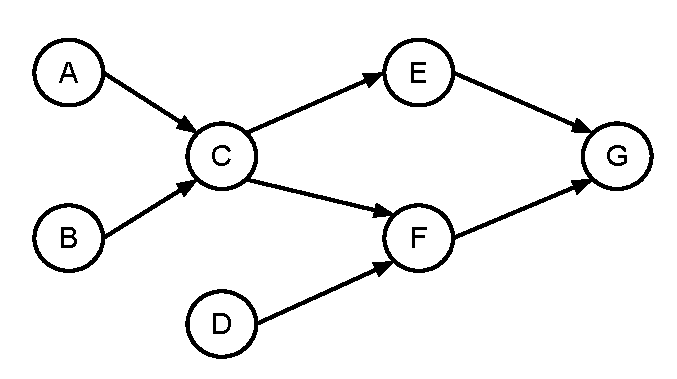
\includegraphics[scale=0.4]{imgs/BNs7n}
\caption{Original DAG}
\end{subfigure}\hfill $\Rightarrow$ \hfill
\begin{subfigure}[H]{0.4\textwidth}
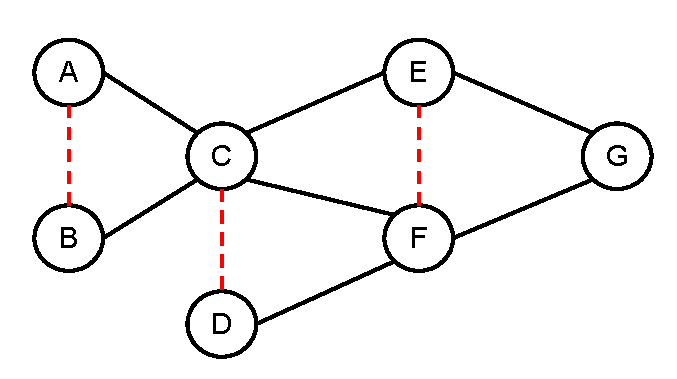
\includegraphics[scale=0.4]{imgs/BNs7nMoral}
\caption{Moral graph}
\end{subfigure}
\end{figure}
\textbf{Moral} is a term known as the married edge of the parents for a collider (two nodes converge at a common node, i.e., non-equivalence ).
\end{frame}
\begin{frame}{Detriangulation of Moral Graph}
\textbf{Note} that the additional dependences are brought by colliders (see nodes C, F, and G) and by conditioned on colliders, dependences will disappear, namely, $A\dep B \, | \, C$ but $A\ci B \,|\, \emptyset$. This motivates us to remove those additional dependences (married edges).\pause
\begin{figure}
\setcounter{subfigure}{0}
\begin{subfigure}[H]{0.4\textwidth}
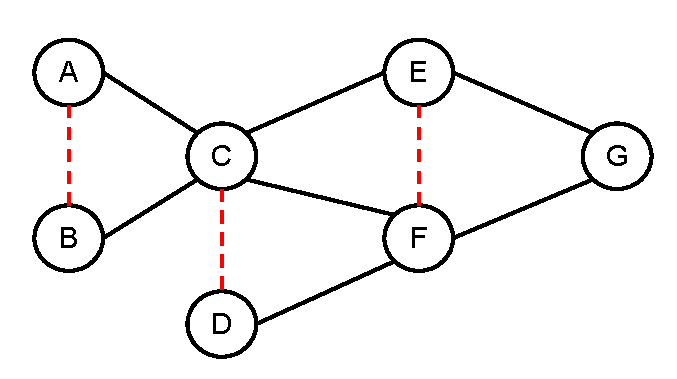
\includegraphics[scale=0.4]{imgs/BNs7nMoral}
\caption{Moral graph}
\end{subfigure}\hfill $\Rightarrow$ \hfill
\begin{subfigure}[H]{0.4\textwidth}
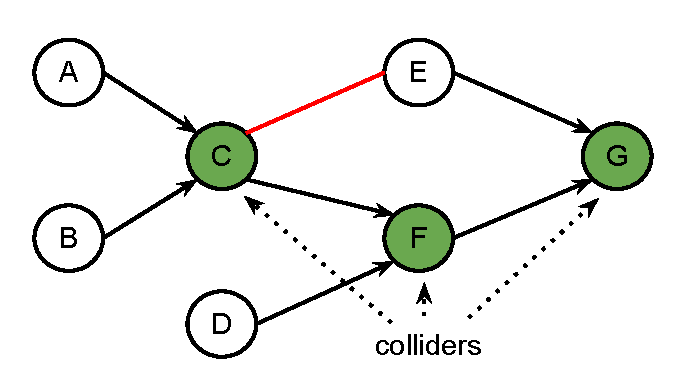
\includegraphics[scale=0.4]{imgs/BNs7nDet}
\caption{Partially directed graph after removing moral edges}
\end{subfigure}
\end{figure}
\end{frame}
\begin{frame}{Contraint Propagation (Judea Pearl 2000)}
Constraints: Colliders, Acyclicity
 \begin{figure}[H]
  \centering
  \hfill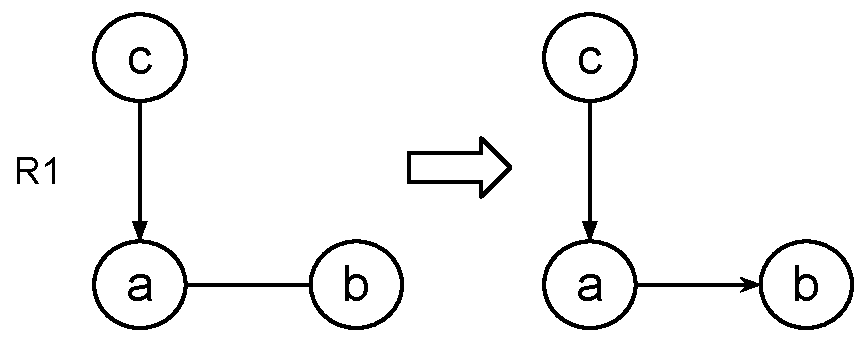
\includegraphics[width=0.4\textwidth]{imgs/R1}%      
  \hfill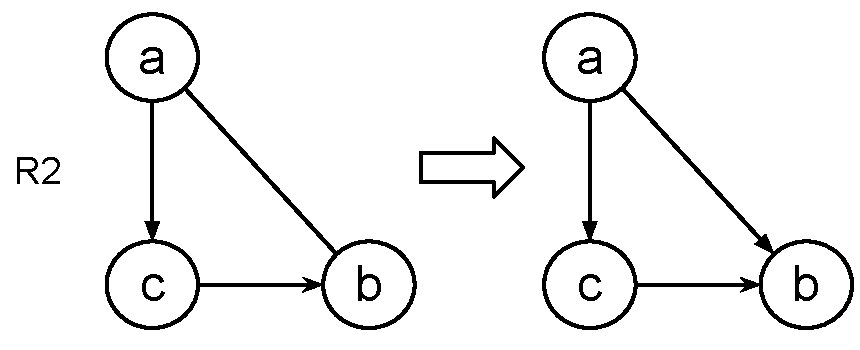
\includegraphics[width=0.4\textwidth]{imgs/R2}\hspace*{\fill}\newline
  \vspace{0.5mm}
  \hspace*{\fill}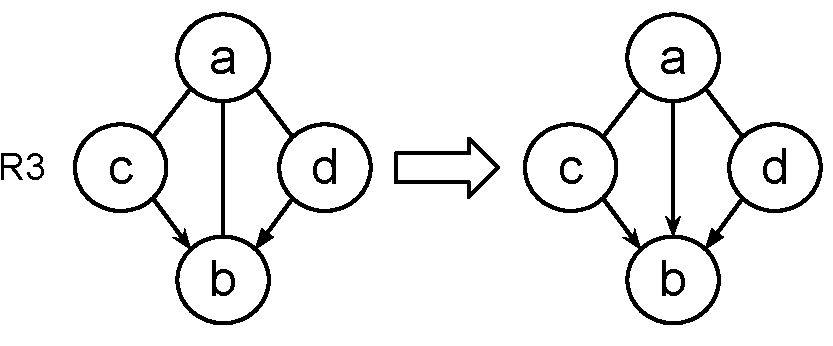
\includegraphics[width=0.4\textwidth]{imgs/R3}%
  \hfill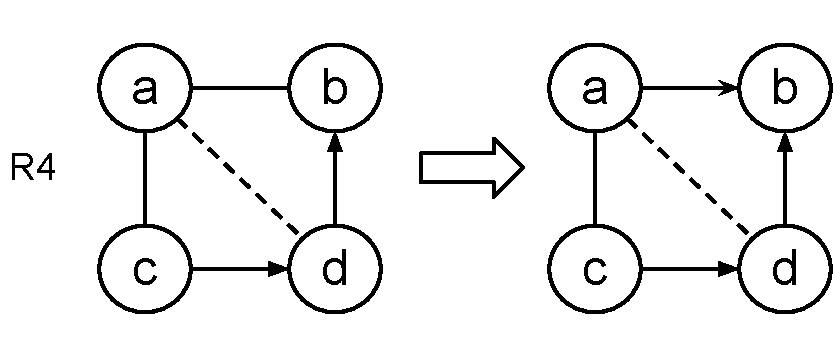
\includegraphics[width=0.4\textwidth]{imgs/R4}\hspace*{\fill}
  \caption{Rules for completion of orientations}
 \end{figure}
\end{frame}
\begin{frame}{Maximally Oriented Acyclic Graph}
Recursively propagate constraints, we obtain a maximally oriented acyclic graph (\alert{only equivalence class})
\begin{figure}
\setcounter{subfigure}{0}
\begin{subfigure}[H]{0.4\textwidth}
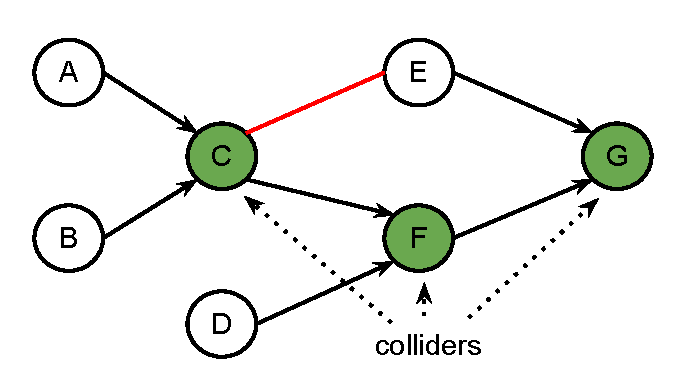
\includegraphics[scale=0.4]{imgs/BNs7nDet}
\caption{Partially directed graph after removing moral edges}
\end{subfigure}\hfill $\Rightarrow$ \hfill
\begin{subfigure}[H]{0.4\textwidth}
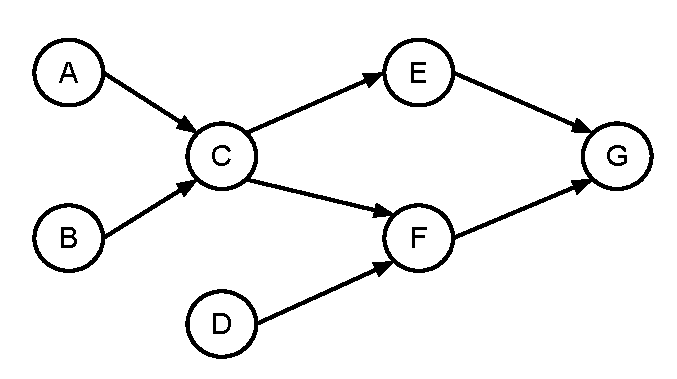
\includegraphics[scale=0.4]{imgs/BNs7n}
\caption{Maximally oriented acyclic graph}
\end{subfigure}
\end{figure}
\end{frame}